% camnotes_test.tex

% comment/uncomment the following to test the various options
%
%\PassOptionsToPackage{blanks}{camnotes}

%\PassOptionsToPackage{noproofs}{camnotes}
%\PassOptionsToPackage{blankproofs}{camnotes}

%\PassOptionsToPackage{noanswers}{camnotes}
%\PassOptionsToPackage{blankanswers}{camnotes}

%\PassOptionsToPackage{student}{camnotes}

%----------------------------------------
\documentclass{article}
%----------------------------------------

\usepackage{camnotes}

% load packages
\usepackage{graphicx}
\usepackage{lipsum}

% document info
\title{Test Document for \texttt{camnotes.sty}}
\author{D Evans \& D McConnell}
\date{Autumn 2017}

% layout
\setlength{\parindent}{0em}
\setlength{\parskip}{0.5em}
\usepackage[a4paper, margin=25mm]{geometry}

% theorem types
\usepackage{ntheorem}
\theoremstyle{break}
\theorembodyfont{\upshape}
\newcounter{theorem}
\newtheorem{theorem}{Theorem}
\newtheorem{definition}[theorem]{Definition}
\newtheorem{lemma}[theorem]{Lemma}
\newtheorem{example}[theorem]{Example}
\newtheorem{exercise}[theorem]{Exercise}
\newtheorem{quiz}[theorem]{Quiz}

% Set stretch factor for blank boxes and images
\setstretchfactor{1} 
\setimagestretchfactor{1} 

% choose colours
\backgroundcolour{yellow!5}
\textcolour{black}
\proofcolour{blue}
\answercolour{red!80}
\solutioncolour{purple}
\showcolour{ForestGreen}

\setboxrule{0.5pt}

\everymath{\displaystyle}
\newcommand{\qed}{\par\hfill$\bigsquare$\par}

%----------------------------------------
\begin{document}
\maketitle
\tableofcontents
\bigskip
\hrule
\begin{center}
This is a test document for the {\tt camnotes.sty} package. The latest version can be found at
\par
\texttt{https://github.com/cardiffmaths/texmf/tex/latex/camnotes}
\end{center}
\hrule

%----------------------------------------
\section{Theorems}

\begin{theorem}\label{thm:test}
This is the statement of the theorem.
\begin{proof}
\lipsum[1-5]
\qed
\end{proof}
\end{theorem}

%The visibility of {\tt proof} environments is controlled by the following package options.
%\bigskip
%\begin{tabular}{ll}
%\hline
%{\tt noproofs}		& print nothing \\
%{\tt blankproofs}	& print blank box \\
%\hline
%\end{tabular}
%\bigskip

%--------------------
\subsection{Examples, exercises and quizzes}
The {\tt example}, {\tt exercise} and {\tt quiz} theorem types are defined in the preamble.

\begin{example}
This is an example.
\end{example}

\begin{exercise}\label{exe:test}
This is an exercise. 
\end{exercise}

\begin{quiz}\label{quiz:test}
This is a quiz. 
\end{quiz}

Examples can have {\tt solutions}.
\begin{example}
Find the integral of $f(x)=x$ over the interval $[0,1]$.
\begin{solution}
$f(x)$ is bounded over $[0,1]$ so 
\[
\int_0^1 x\,dx = \left[\frac{x^2}{2}\right]_0^1 = \frac{1}{2}
\]
\end{solution}
\end{example}

The same result be achieved using the {\tt blankbox} environment, but without the heading.
\begin{example}
Find the integral of $f(x)=x$ over the interval $[0,1]$.
\begin{blankbox}
$f(x)$ is bounded over $[0,1]$ so 
\[
\int_0^1 x\,dx = \left[\frac{x^2}{2}\right]_0^1 = \frac{1}{2}
\]
\end{blankbox}
\end{example}



%----------------------------------------
\section{Question types (adapted from \texttt{exam.cls})}
%----------------------------------------

\verb+\ans+ commands and {\tt answer} environments can be inserted anywhere. Their visibility is controlled by the following package options.

\bigskip
\begin{tabular}{ll}
\hline
{\tt blankanswers}	& print blank box \\
{\tt noanswers}		& print nothing \\
\hline
\end{tabular}
\bigskip

Here is an answer (it might not be visible):
\begin{answer}
%But what is the question?
\lipsum[1]
\end{answer}

We can force answers to be included using \verb+\answerson ... \endanswerson+. The following answer will always be included.
\answerson
\begin{answer}
This is always included
\end{answer}
\endanswerson

We can force answers to be excluded using  \verb+\answersoff ... \endanswersoff+. The following answer will never be included.
\answersoff
\begin{answer}
This is never included
\end{answer}
\endanswersoff

%--------------------
\subsection{Questions, parts and subparts}

Here is an exercise containing a {\tt questions} environment, which itself contains a {\tt parts} environment. 
\begin{exercise}\label{exe:demo}
\begin{questions}
\question First question.
\begin{parts}
\part First part.
\ans{Answer to the first part.}
\part Second part.
\begin{subparts}
\subpart First subpart.
\ans{Answer to the first subpart.}
\subpart Second subpart.
\ans{Answer to the second subpart.}
\end{subparts}
\end{parts}
\question Second question.
\ans{Answer to the second question.}
\end{questions}
\end{exercise}

%--------------------
\subsection{Multiple choice and multiple answer questions}

The following quiz has two multiple choice questions (\texttt{choices}), two multiple answer questions (\texttt{checkboxes}) questions, and a free-text question (default).

\begin{quiz}
\begin{questions} 

% true or false (implemented using multiple choice)
\question Necessity is the mother of invention.
\begin{choices}
\correctchoice True 		
\choice False		
\end{choices}

% multiple choice question
\question In what year did Columbus first cross the Atlantic?
\begin{choices}
\choice 1490 %\begin{response} Sorry, better luck next time.\end{response}
\choice 1491 %\begin{response} Sorry, better luck next time.\end{response}
\correctchoice   1492 %\begin{response} Correct, well done.\end{response} 
\choice 1493 %\begin{response} Sorry, better luck next time.\end{response}
\end{choices}
\begin{answer}
In 1492, Columbus sailed the ocean blue.
\end{answer}

% multiple answer question 
\question
\label{qu:series}
Which of the following series converge?
\begin{checkboxes}
\choice $\sum_{n=1}^{\infty}\frac{1}{n}$
\correctchoice $\sum_{n=1}^{\infty}\frac{1}{n^2}$
\correctchoice $\sum_{n=1}^{\infty}\frac{1}{n^4}$
\end{checkboxes}
\begin{answer}
\begin{itemize}
\item $\sum_{n=1}^{\infty}\frac{1}{n}$ diverges (this is the harmonic series). 
\item $\sum_{n=1}^{\infty}\frac{1}{n^2} = \pi^2/6$.
\item $\sum_{n=1}^{\infty}\frac{1}{n^4} = \pi^4/90$.
\end{itemize}
\end{answer}

% free text
\question 
Write a short essay on a topic of your choice.  
\begin{answer}
Anything sensible will do.
\end{answer}

\end{questions}
\end{quiz}


%----------------------------------------
\section{Blanks}
%----------------------------------------

\subsection{Blank (inline)}
The words `red' and `'blue' are enclosed in \verb+\blank+ commands. These are controlled by the \verb+blanks+ option.

Roses are \blank{red}, violets are \blank{blue}.

\subsection{Blankboxes}
Here is a blankbox.
\begin{blankbox}
\lipsum[1]
\end{blankbox}

\subsection{Solutions}
Here is a solution.
\begin{solution}
\lipsum[2]
\end{solution}

\subsection{Proofs}
Here is a proof (might be invisible).
\begin{proof}
\lipsum[3]
\end{proof}

\subsection{Answers}
Here is an answer (might be invisible).
\begin{answer}
\lipsum[4]
\end{answer}


As with any environment, these environments can be delimited as follows:
\begin{verbatim}
\blankbox
Content to be blanked out in student workbooks.
\endblankbox
\end{verbatim}

%----------------------------------------
\section{Images}
Here is an image on its own (never hidden).
\begin{center}
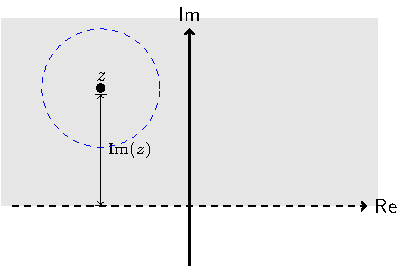
\includegraphics[scale=1]{upperhalf_full}
\end{center}

Here is the image in a blankbox.
\begin{blankbox}
\begin{center}
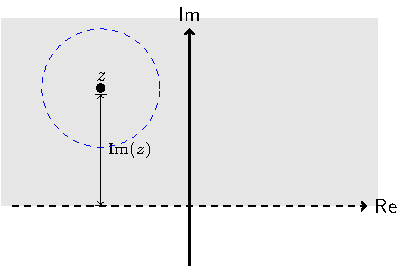
\includegraphics[scale=1]{upperhalf_full}
\end{center}
\end{blankbox}

Here is the image in a solution.
\begin{solution}
\begin{center}
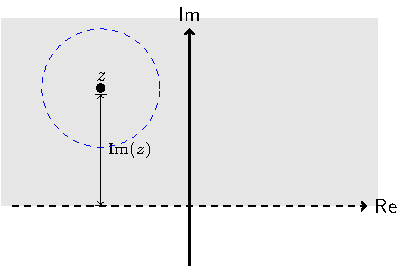
\includegraphics[scale=1]{upperhalf_full}
\end{center}
\end{solution}

Here is the image in a proof (might be invisible).
\begin{proof}
\begin{center}
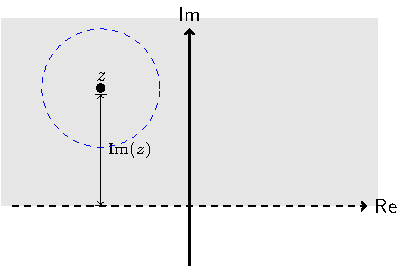
\includegraphics[scale=1]{upperhalf_full}
\end{center}
\end{proof}

Here is the image in an answer (might be invisible).
\begin{answer}
\begin{center}
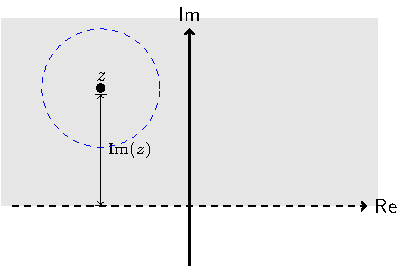
\includegraphics[scale=1]{upperhalf_full}
\end{center}
\end{answer}

\subsection{Altgraphics}

The \verb+\altgraphics+ command can be used to print a partial image in the student version and a complete image in the full version. 

Here is the (partial) image in a blankbox.
\begin{blankbox}
\begin{center}
\altgraphics[scale=1]{upperhalf_full}{upperhalf_partial}
\end{center}
\end{blankbox}

Here is the (partial) image in a solution.
\begin{solution}
\begin{center}
\altgraphics[scale=1]{upperhalf_full}{upperhalf_partial}
\end{center}
\end{solution}

Here is the (partial) image in a proof (might be invisible).
\begin{proof}
\begin{center}
\altgraphics[scale=1]{upperhalf_full}{upperhalf_partial}
\end{center}
\end{proof}

Here is the (partial) image in an answer (might be invisible).
\begin{answer}
\begin{center}
\altgraphics[scale=1]{upperhalf_full}{upperhalf_partial}
\end{center}
\end{answer}

%--------------------
\subsection{TikZ pictures}

% define picture
\tikzset{every picture/.style={line width=1pt}}
\tikzset{
    circles/.pic={
        \draw[Green] (0,0) circle (0.5);
        \draw[Blue] (0,0) circle (1);
        \draw[Red] (0,0) circle (1.5);
        \draw[Black] (0,0) circle (2);
    }
}
\tikzset{
    squares/.pic={
        \draw[Green] (-0.5,-0.5) rectangle (0.5,0.5);
        \draw[Blue]  (-1,-1) rectangle (1,1);
        \draw[Red]   (-1.5,-1.5) rectangle (1.5, 1.5);
        \draw[Black] (-2,-2) rectangle (2,2);
    }
}
\tikzset{
    circlesandsquares/.pic={
        \pic{circles};
        \pic{squares};
    }
}

Here are some circles and squares. These are never hidden.
\begin{center}
\tikz\pic{circlesandsquares};
\end{center}

Here is a \verb+blankbox+ containig the circles. We have to include \verb+\blanktikz+ explicitly.
\begin{blankbox}
\blanktikz
Here are some circles.
\begin{center}
\tikz\pic{circles};
\end{center}
\end{blankbox}

Here is an \verb+answerbox+ containig the squares. We have to include \verb+\blanktikz+ explicitly.
\begin{answer}
\blanktikz
Here are some squares.
\begin{center}
\tikz\pic{squares};
\end{center}
\end{answer}

Here are some circles and squares. Back to normal?
\begin{center}
\tikz\pic{circlesandsquares};
\end{center}

%========================================
\end{document}
%========================================


